\label{ch:experimental_results}

\section{FTIR}
Here are presented the FTIR spectra of a raw, ground and polished sample. 

\begin{figure}[H]
    \centering
    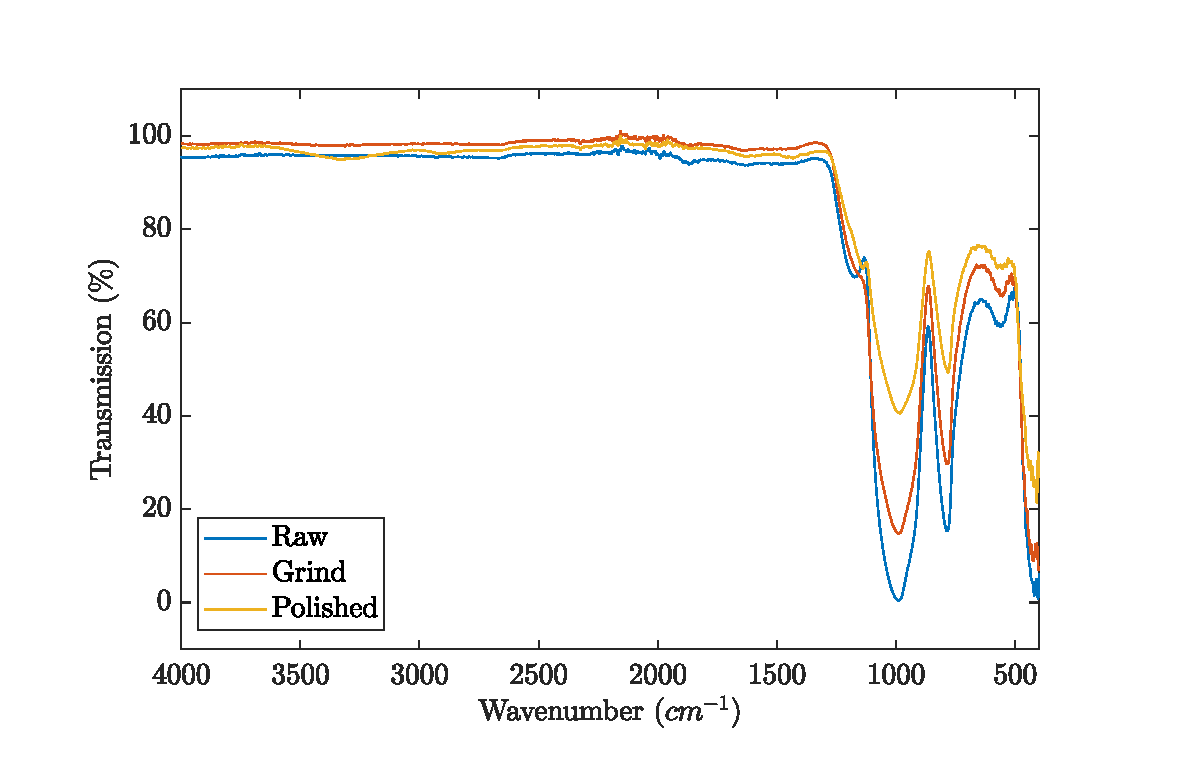
\includegraphics[width = \textwidth]{chapter_5/others/ftir_plot.pdf} 
    \vspace*{-30pt}
    \caption{FTIR spectra.}
    \label{fig:ftir_plot}
 \end{figure}
 As already said in Chapter~\ref{fig:ftir_issues} the differences in amplitude is not relevant for a measurement but only the position and presence of transmission dips. 
\\
From Figure~\ref{fig:table_inorganic} we can identify that the two major peaks present in the spectra, at $1000 \:cm^{-1} $and $780 \:cm^{-1}$, respectively corresponds to \ce{SiO2} and \ce{SiO3} compounds, obviously present in glass.
\\
The small dip at $1173 \:cm^{-1}$ is associated to \ce{C-O} stretching and could be caused by ethanol, which was used to clean the sample between measurements. 
\\
Due to the fact that the all the contaminants present at the surface of glass are inorganic, they cannot be detected by FTIR. We performed the measurements to check if organic compounds were also deposited on the samples.

\section{Contact Angle Measurement}
Contact angle measurements were also performed on the raw and on a polished sample. The results are presented in the next figure.
\begin{figure}[H]
    \centering
    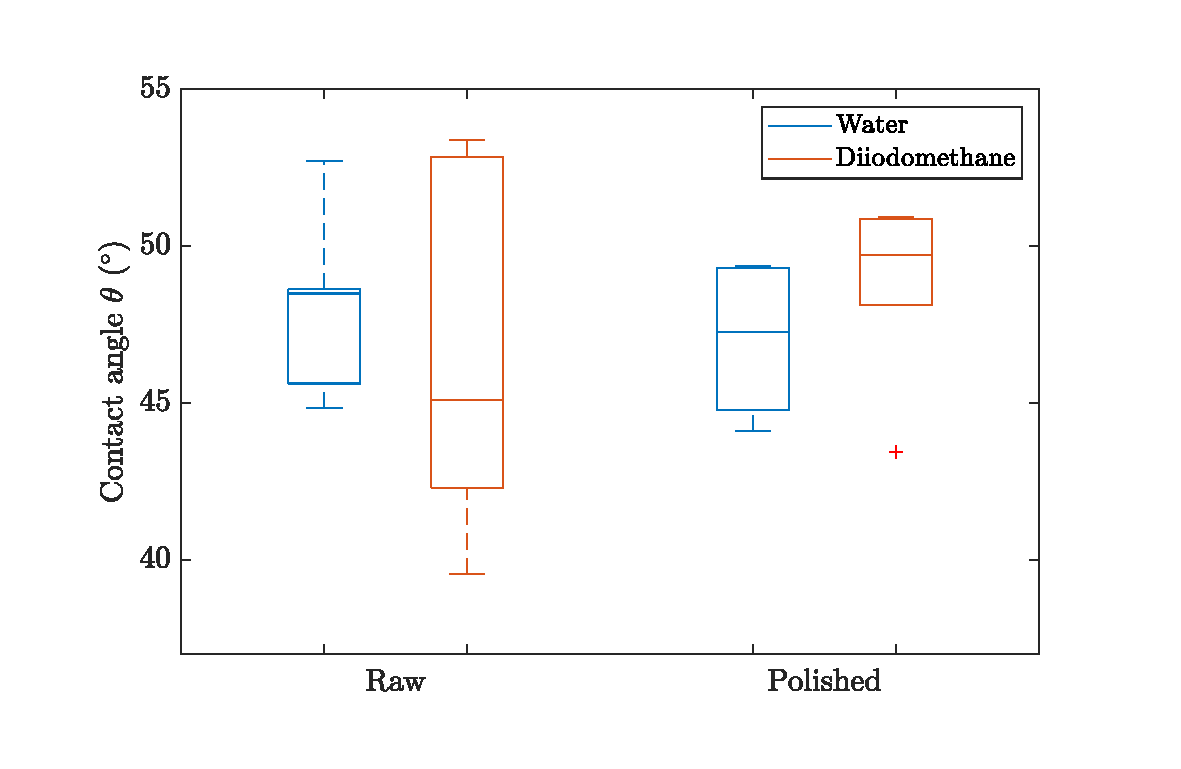
\includegraphics[width = \textwidth]{chapter_5/others/contact_angle.pdf} 
    \vspace*{-30pt}
    \caption{Contact angle measurements for a raw and a polished sample. }
    \label{fig:contact_angle_raw_polished}
 \end{figure}
Considering the shifts in the average value of the measured angle between the polar and the non-polar probe liquids, there could be a change in the contributions to the surface energy of the glass. Nevertheless, due the high error in the measurements of the raw sample, no real conclusions can be drawn.

\section{LIBS}
\label{sec:LIBS_measurements}

In this section are presented the experimental results of the LIBS measurements, as well as the fitting to the theoretical concentrations.
\\
In 

\subsection{Data Fitting Method}
\label{subsec:data_fitting}
As already explained in detail in Chapter~\ref{sec:theoretical_prediction}, if normal diffusion is the primary driving mechanism for the presence of contaminants in the glass, the expected concentration of contaminants should follow Equation~\ref{eq:c_bar_equation}.
\\
In the expression there are three different parameters that can influence the behavior of the function: $d_a$, $C_0$ and $D$. They are, respectively, the ablation depth of the LIBS measurement, the saturation concentration and the diffusion constant.
\\
The ablation depth should be the same for every measurement we performed, as it only depends on the laser parameters and on the target material, both of which were constant for all the experiments.
\\
To estimate this parameter we have performed some depth analyses with a 3D microscope to a pure silica sample that was ablated five different times with the same laser energy of $15 \: mJ$ but with an increasing number of pulses, from 5 to 25.

\begin{figure}[H]
    \centering
    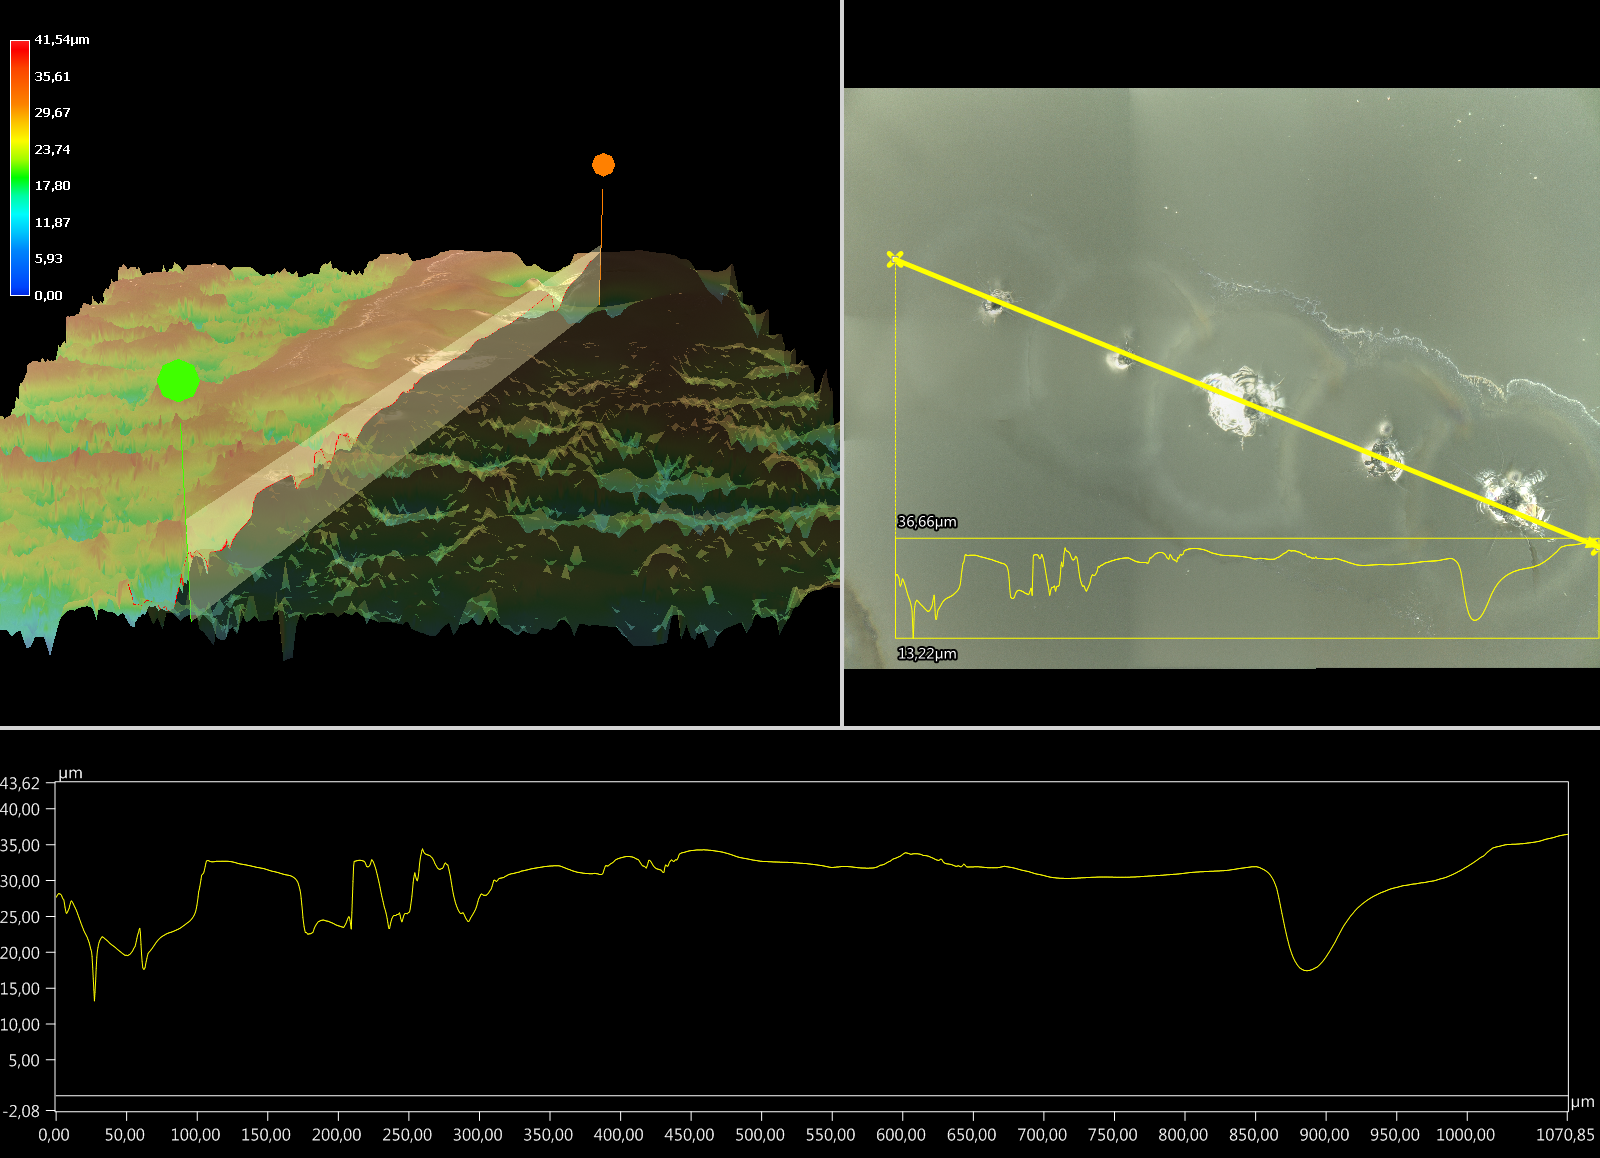
\includegraphics[width = 0.8\textwidth]{chapter_5/LIBS/data_fit/3dmicroscope_profile.png} 
    \caption{Width and depth measurements of LIBS craters performed with a 3D microscope. The peaks are ordered from left to right accordingly to the number of pulses.}
    \label{fig:3d_microscope_craters}
 \end{figure}

 Unfortunately, due to the translucency of silica glass, optical measuring methods cannot be fully trusted, especially when performing depth profiling. The information presented in Figure~\ref{fig:3d_microscope_craters} is only useful to give an idea of the order or magnitude of the value.
 \\
For the first two peaks, the ones corresponding to 5 and 10 pulses, the depth measured by the microscope is around $5 \: \mu m$. In the case of our experiments the energy was the same but only one pulse was performed, with consequently less ablation. As an estimation of the crater depth, we considered the value cited before but one order of magnitude lower, $d_a = 0.5 \: \mu m$.
\\
The two other parameters, $C_0$ and $D$, strictly depend on the specific characteristics of the diffusion.
\\
The of magnitude for $D$ in glasses can be found in literature; in [paper aluminum in glass] there is an estimation of the diffusion coefficient of gaseous metallic aluminum into the amorphous silica layer that forms on top of silicon wafers. The value is given by the following equation:
\begin{align}
    D/m^2s^{-1} = 1.83 \cdot 10^{-13}\exp \left(\frac{-1.12 \cdot 10^5}{RT}\right) \label{eq:diffiusion_coef_aluminum}
\end{align}
Where $R$ is the ideal gas constant and $T$ is the absolute temperature of the chamber. This expression is valid for values of the temperature between 973 and $1173 \:K$. By taking the middle value of that range, the corresponding $D$ is equal to $2.02 \cdot 10^{-18} \:m^2s^{-1}$.
\\
Regarding $C_0$, for the fitting procedure to make sense, the value of the parameter should be of the order of the experimental values; ideally, if the measurements follow a curve similar to the one in Figure~\ref{fig:c_bar_mixed}, the value of $C_0$ should be the one corresponding to the concentrations of the values taken at later polishing times.
\\
For the actual fitting, we employed a simple algorithm. We defined two arrays with the possible values of $D$ and $C_0$: for $D$ we constructed a logarithmic space between $10^{-20}$ and $10^{-7}$, while for $C_0$ we built a linear space between the minimum and two times the maximum the measured concentration of the element we were trying to fit.
\\
We then constructed another array with all the possible combinations between the two parameters, and, finally, we identified the couple that resulted in the least round mean square (rms) of the difference between the theoretical function and the data.
\\
The whole procedure should be enough to perform qualitative comparisons between different species.





\subsection{Concentration of the Polishing Solution}
\label{subsec:conc_results}
In the next section we will display all the collected data. Initially, for each polish concentration, a qualitative comparison of the notable wavelength ranges between the spectra of the raw, ground and polished sample is shown. Secondly, the plots with the measured contaminants concentrations are presented. The diffusion parameters fitted with the method proposed in the previous section are also shown. Lastly, we will exhibit the differences between the measured contaminants relatively to the polish suspension concentration.
\\
\subsubsection{Polish Concentration: 5pc}
\label{subsubsec:5pc}
\vspace*{-25pt}
\begin{figure}[H]
    \centering
    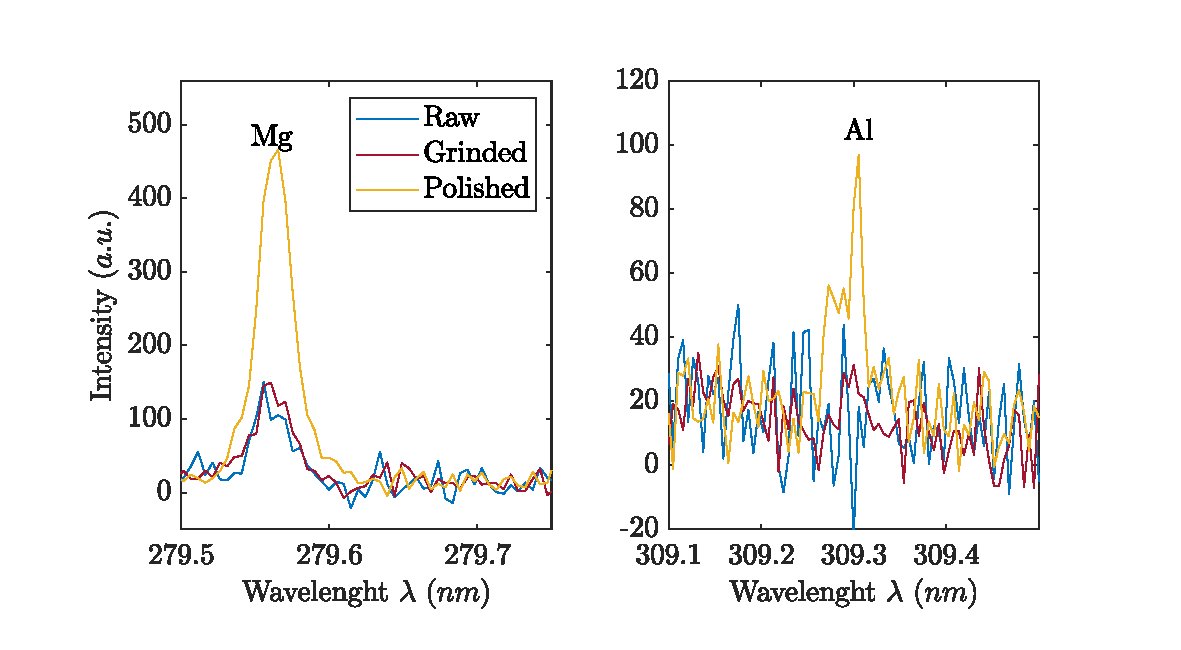
\includegraphics[width = \textwidth]{chapter_5/LIBS/spectra_comparison/tap_5pc_first.pdf} 
    %\caption{Width and depth measurements of LIBS craters performed with a 3D microscope. The peaks are ordered from left to right accordingly to the number of pulses.}
    %\label{fig:3d_microscope_craters}
 \end{figure}

\vspace*{-68pt}
\begin{figure}[H]
    \centering
    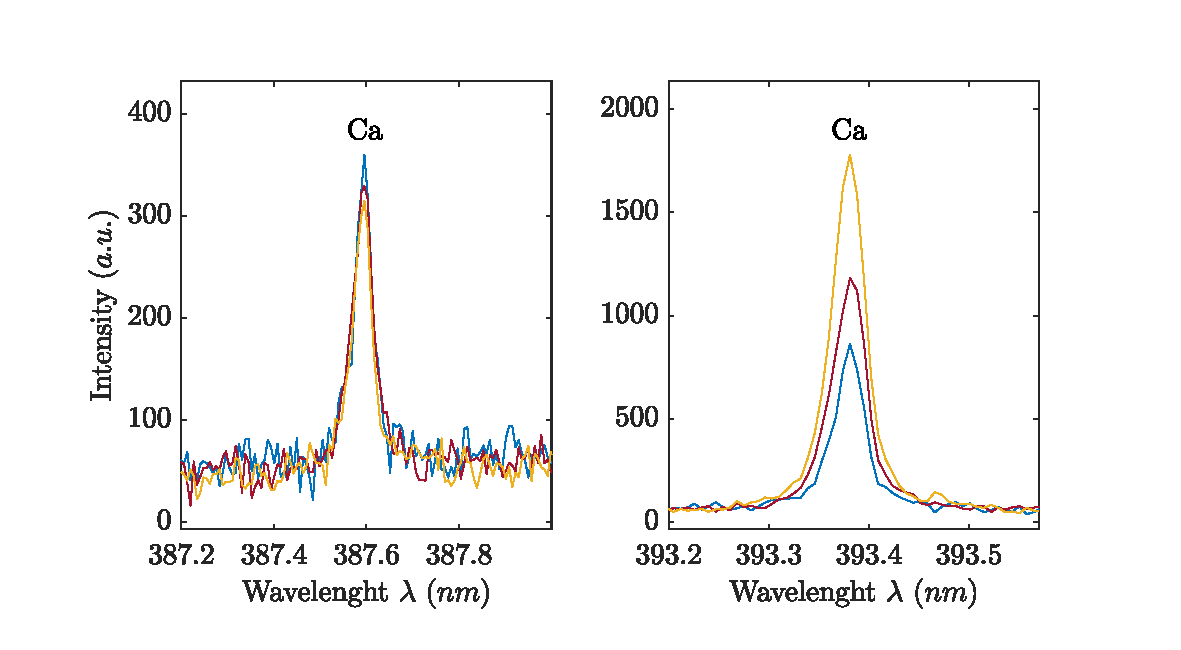
\includegraphics[width = \textwidth]{chapter_5/LIBS/spectra_comparison/tap_5pc_second.pdf} 
    %\caption{Width and depth measurements of LIBS craters performed with a 3D microscope. The peaks are ordered from left to right accordingly to the number of pulses.}
    %\label{fig:3d_microscope_craters}
 \end{figure}

\vspace*{-68pt}
\begin{figure}[H]
    \centering
    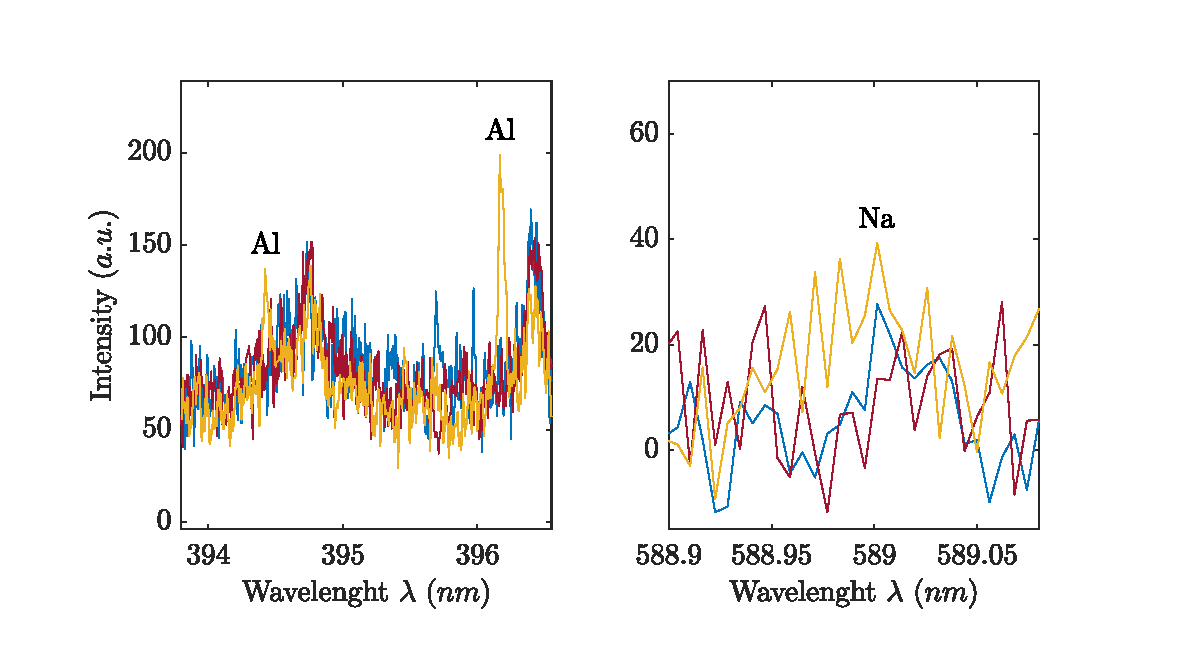
\includegraphics[width = \textwidth]{chapter_5/LIBS/spectra_comparison/tap_5pc_third.pdf} 
    %\caption{Width and depth measurements of LIBS craters performed with a 3D microscope. The peaks are ordered from left to right accordingly to the number of pulses.}
    %\label{fig:3d_microscope_craters}
 \end{figure}

 As it can be seen from the plots, the polished sample can be easily distinguished from the other two spectra; in particular, the aluminum peaks are present only in the polished sampled, while the other elements are found also in the raw and ground spectra. Due to the lower sensitivity of the detector in the visible range, the sodium peak cannot be easily distinguished from the noise floor. Its presence is expected since, as shown in Table~\ref{table:water_composition}, a non-negligible quantity is dissolved in the water. Moreover, sodium has a low LOD and should be easily detectable with LIBS.
\\
For the next series of graphs, only the time evolution of the polishing phase is shown.
\begin{figure}[H]
    \centering
    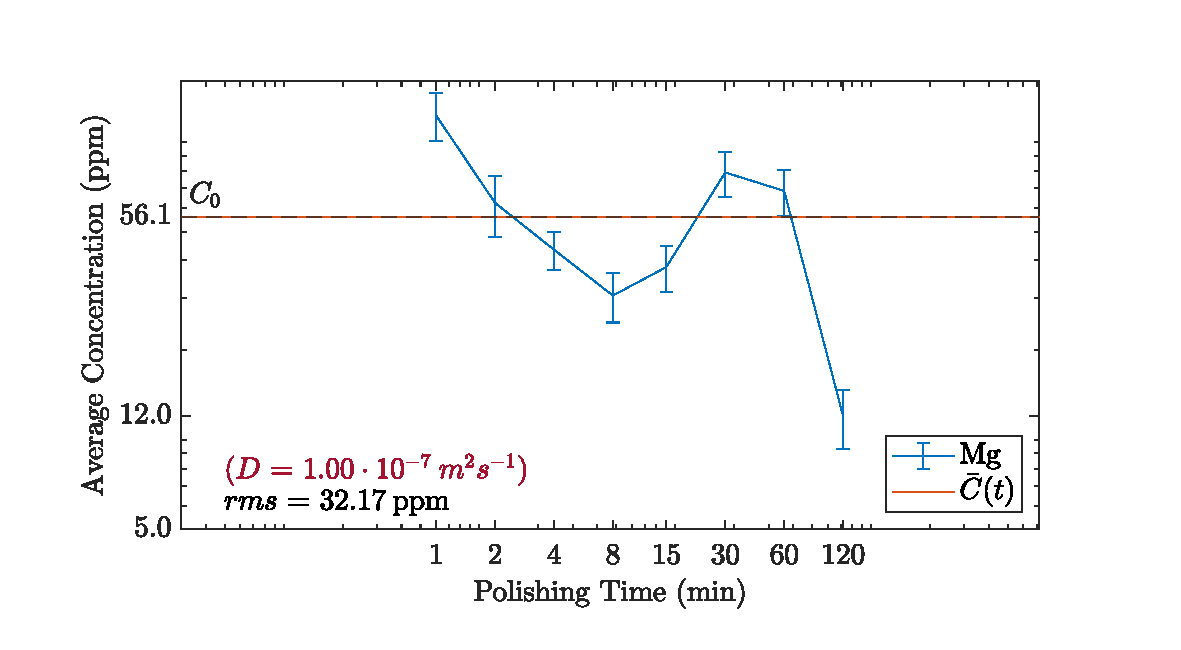
\includegraphics[width = \textwidth]{chapter_5/LIBS/data_fit/fit_tap_5pc_Mg.pdf} 
    %\caption{Width and depth measurements of LIBS craters performed with a 3D microscope. The peaks are ordered from left to right accordingly to the number of pulses.}
    %\label{fig:3d_microscope_craters}
 \end{figure}
\vspace*{-48pt}
 \begin{figure}[H]
    \centering
    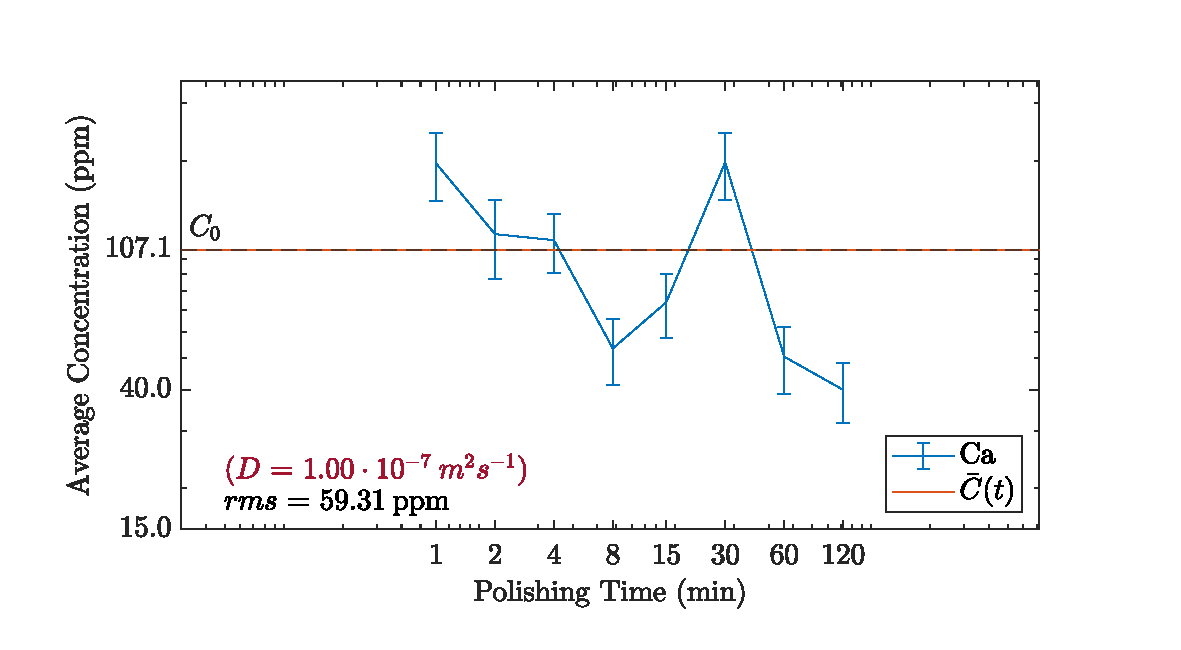
\includegraphics[width = \textwidth]{chapter_5/LIBS/data_fit/fit_tap_5pc_Ca.pdf} 
    %\caption{Width and depth measurements of LIBS craters performed with a 3D microscope. The peaks are ordered from left to right accordingly to the number of pulses.}
    %\label{fig:3d_microscope_craters}
 \end{figure}
 \begin{figure}[H]
    \centering
    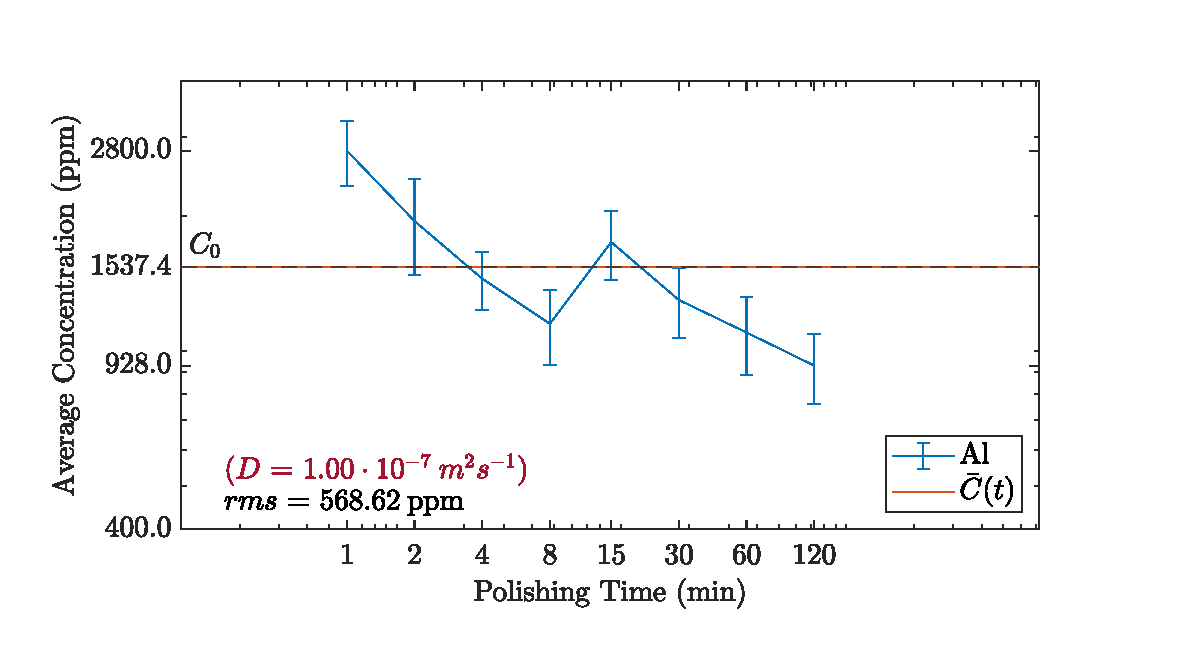
\includegraphics[width = \textwidth]{chapter_5/LIBS/data_fit/fit_tap_5pc_Al.pdf} 
    %\caption{Width and depth measurements of LIBS craters performed with a 3D microscope. The peaks are ordered from left to right accordingly to the number of pulses.}
    %\label{fig:3d_microscope_craters}
 \end{figure}

    \vspace*{-20pt}
 \begin{figure}[H]
    \centering
    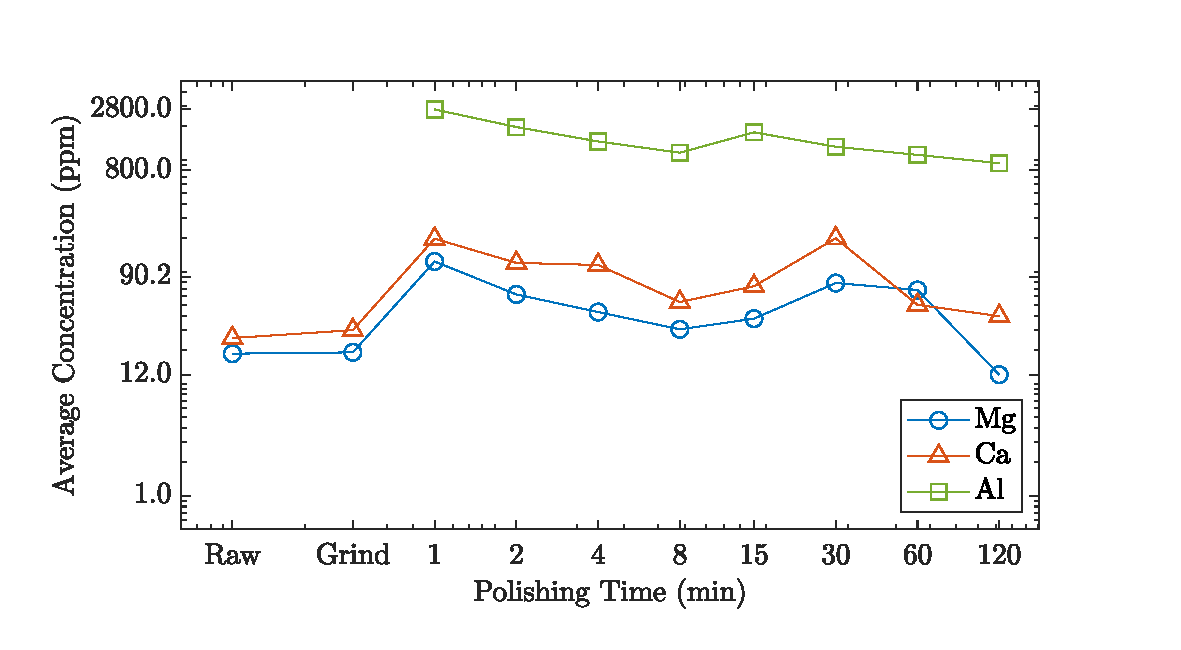
\includegraphics[width = \textwidth]{chapter_5/LIBS/Tap_elem_comparisons/Tap_elements_5_pc.pdf} 
    \vspace*{-30pt}
    \caption{Comparison of the concentration values of the major contaminants as a function of the polishing time, for the glass polished with a 5pc suspension.}
    \label{fig:tap_elem_5pc}
 \end{figure}
 In Figure~\ref{fig:tap_elem_5pc} it is clear that all the elements share a similar decreasing behavior.





\pagebreak



\subsubsection{Polish Concentration: 15pc}
\label{subsubsec:15pc}
\vspace*{-25pt}
\begin{figure}[H]
    \centering
    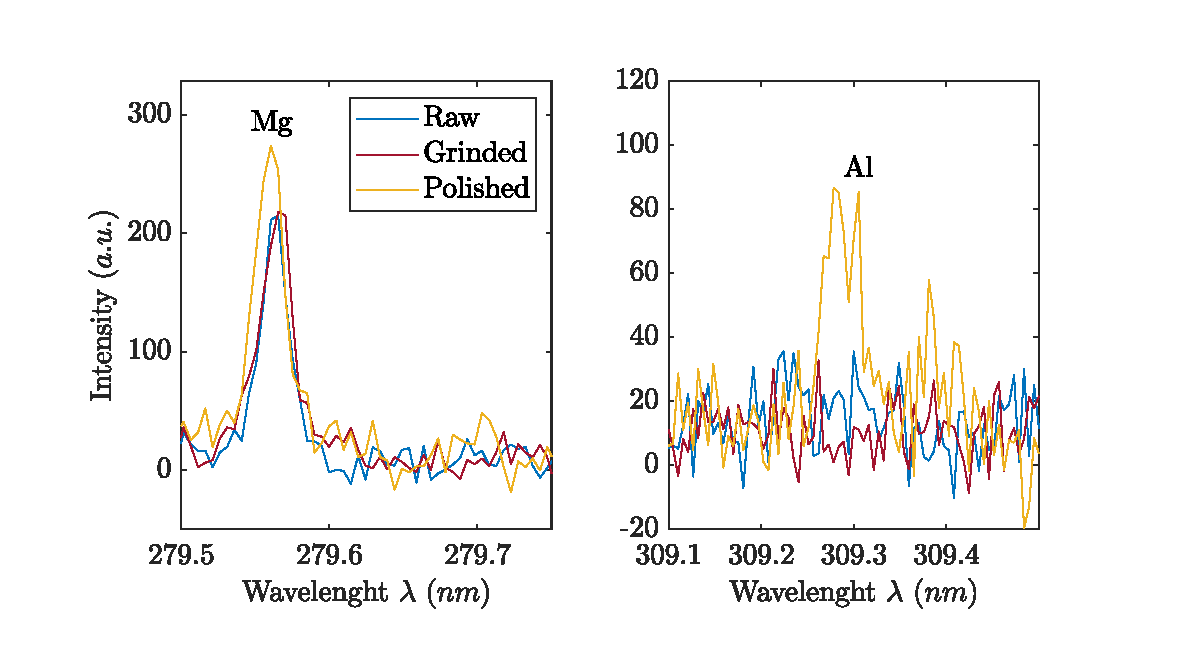
\includegraphics[width = \textwidth]{chapter_5/LIBS/spectra_comparison/tap_15pc_first.pdf} 
    %\caption{Width and depth measurements of LIBS craters performed with a 3D microscope. The peaks are ordered from left to right accordingly to the number of pulses.}
    %\label{fig:3d_microscope_craters}
 \end{figure}

\vspace*{-68pt}
\begin{figure}[H]
    \centering
    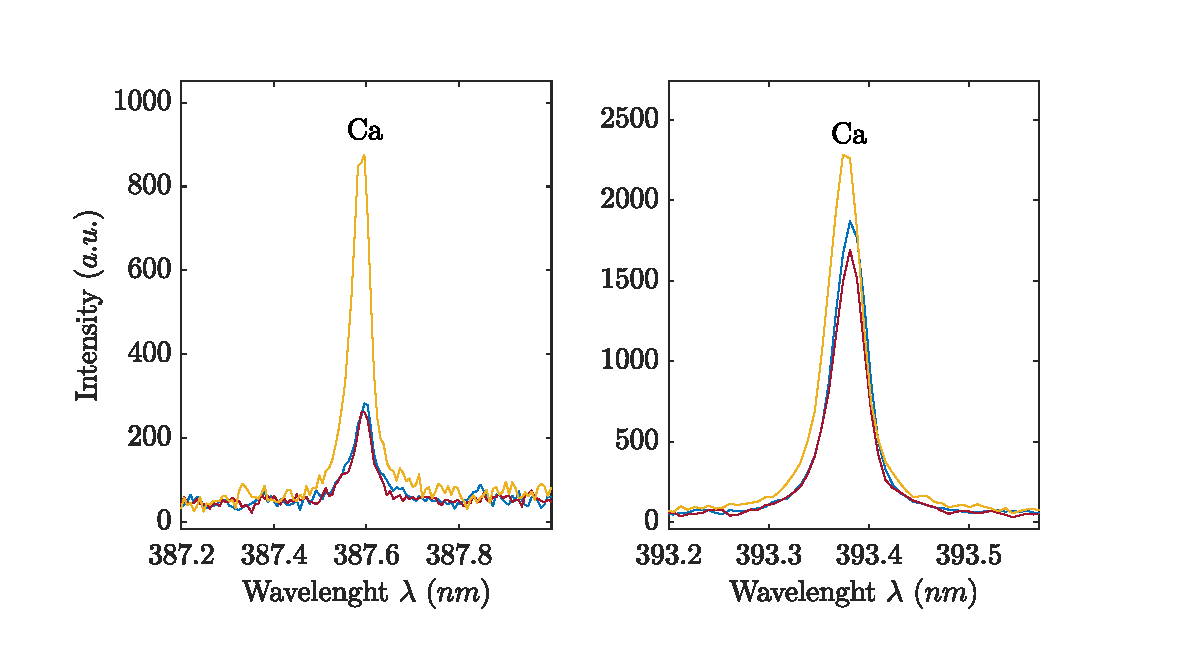
\includegraphics[width = \textwidth]{chapter_5/LIBS/spectra_comparison/tap_15pc_second.pdf} 
    %\caption{Width and depth measurements of LIBS craters performed with a 3D microscope. The peaks are ordered from left to right accordingly to the number of pulses.}
    %\label{fig:3d_microscope_craters}
 \end{figure}

\vspace*{-68pt}
\begin{figure}[H]
    \centering
    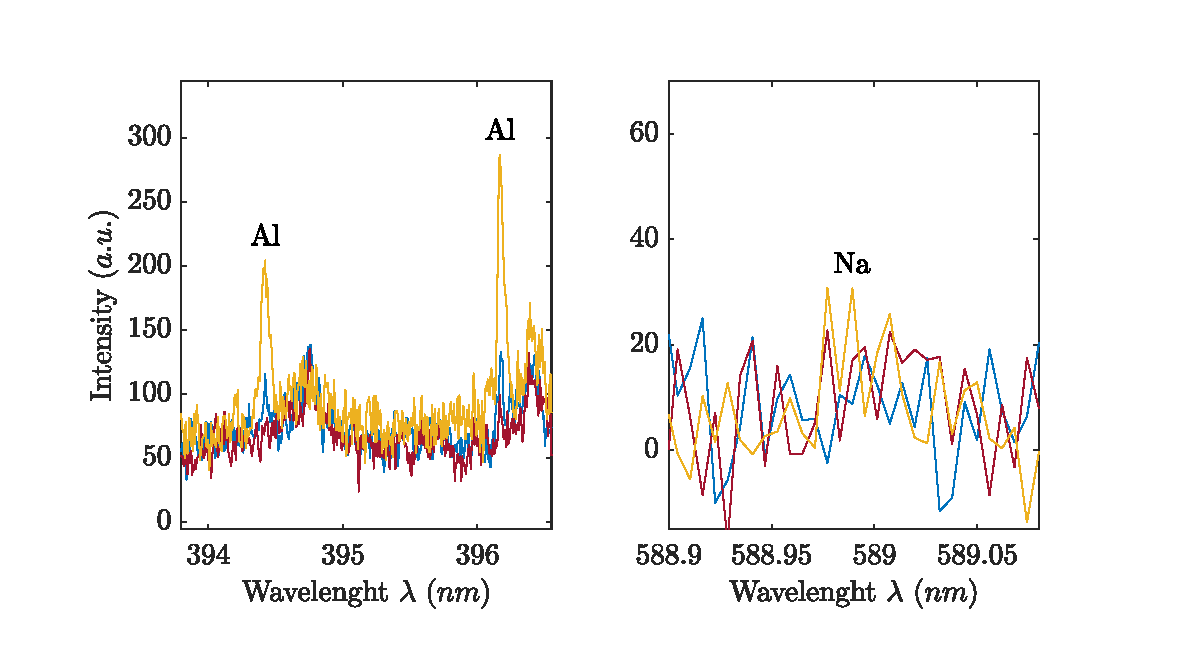
\includegraphics[width = \textwidth]{chapter_5/LIBS/spectra_comparison/tap_15pc_third.pdf} 
    %\caption{Width and depth measurements of LIBS craters performed with a 3D microscope. The peaks are ordered from left to right accordingly to the number of pulses.}
    %\label{fig:3d_microscope_craters}
 \end{figure}

 The behavior of the spectra is similar to the 5pc case. The most notable difference is the in the \ce{Ca} peaks, where in this case, the difference between the polished and unpolished sample is more relevant in the peak located at a  smaller wavelength. This could probably be related to differences in the characteristics of the plasma, like temperature and electron density.

\begin{figure}[H]
    \centering
    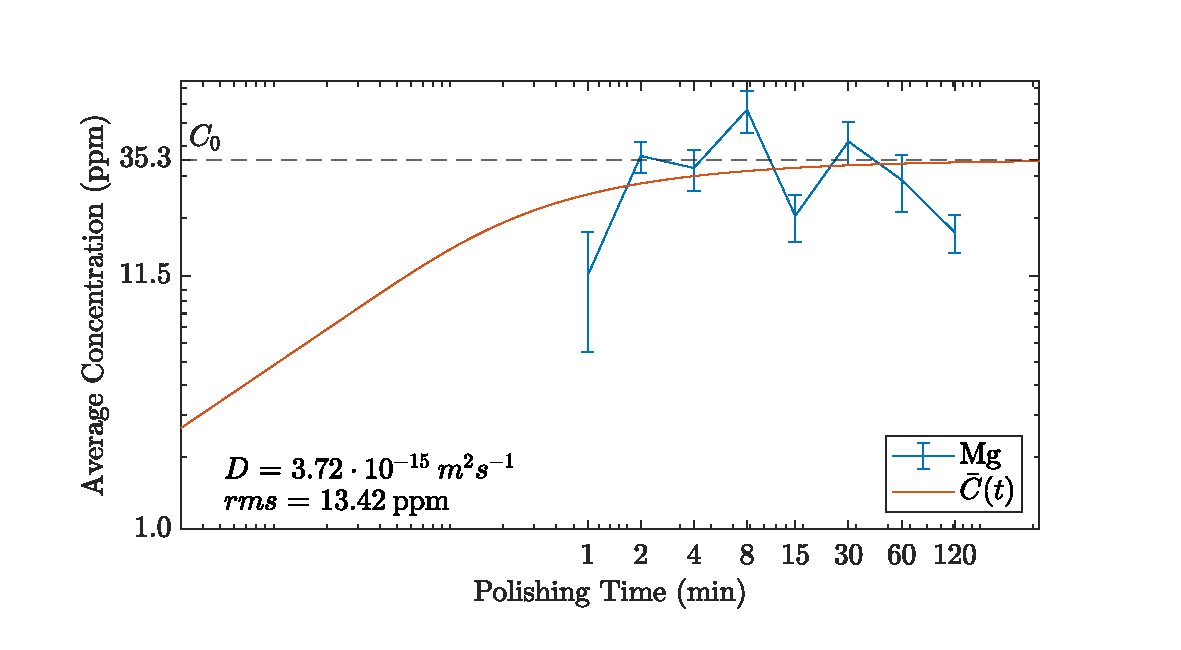
\includegraphics[width = \textwidth]{chapter_5/LIBS/data_fit/fit_tap_15pc_Mg.pdf} 
    \vspace{-30pt}
    \caption{Measurement for the Mg concentration fitted to the diffusion model.}
    \label{fig:fit_tap_15pc}
 \end{figure}

 \begin{figure}[H]
    \centering
    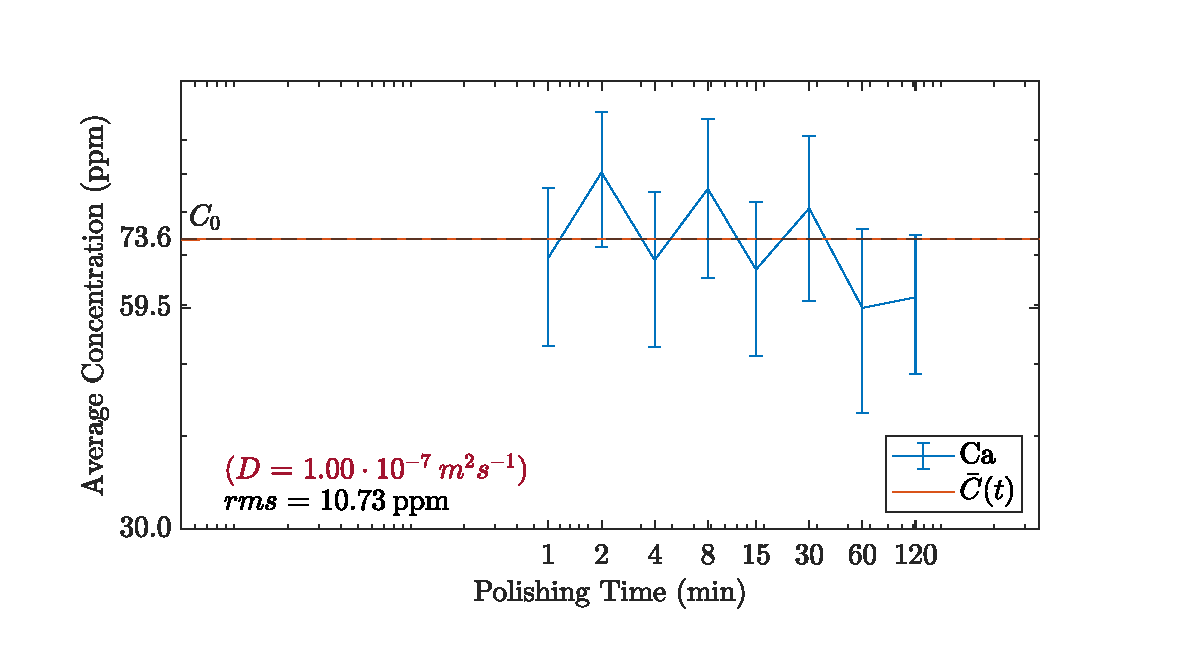
\includegraphics[width = \textwidth]{chapter_5/LIBS/data_fit/fit_tap_15pc_Ca.pdf} 
    %\caption{Width and depth measurements of LIBS craters performed with a 3D microscope. The peaks are ordered from left to right accordingly to the number of pulses.}
    %\label{fig:3d_microscope_craters}
 \end{figure}
    \vspace{-40pt}
 \begin{figure}[H]
    \centering
    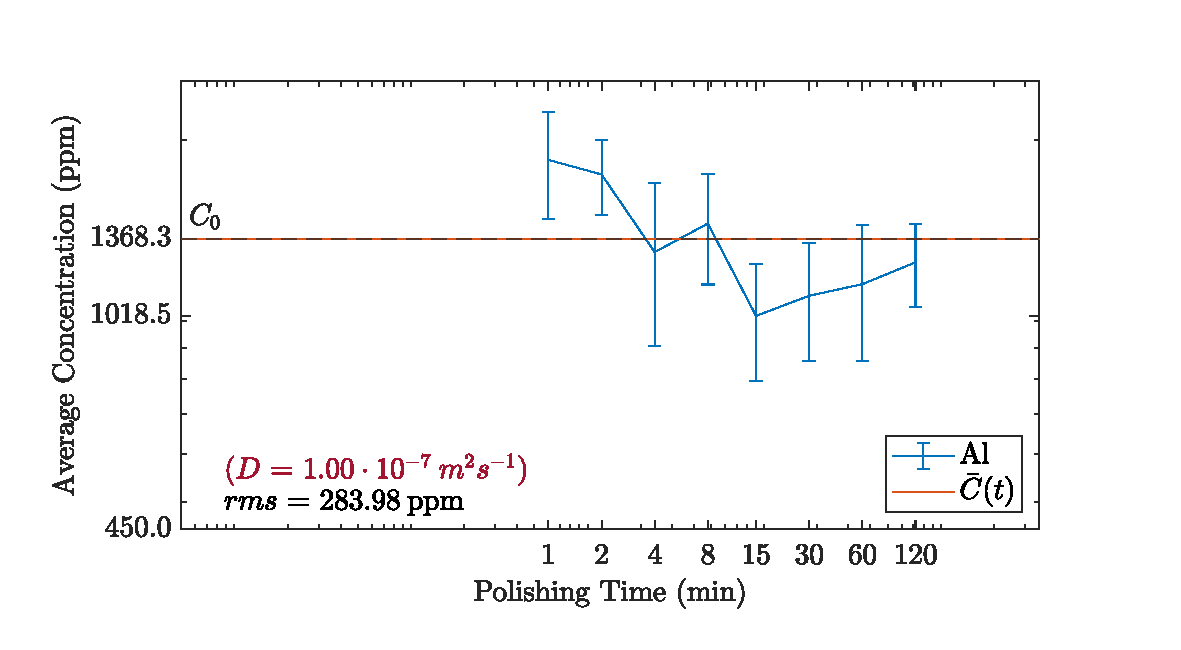
\includegraphics[width = \textwidth]{chapter_5/LIBS/data_fit/fit_tap_15pc_Al.pdf} 
    %\caption{Width and depth measurements of LIBS craters performed with a 3D microscope. The peaks are ordered from left to right accordingly to the number of pulses.}
    %\label{fig:3d_microscope_craters}
 \end{figure}

 \vspace{-20pt}

 As can be seen from Figure~\ref{fig:fit_tap_15pc}, in this case, the data could be fairly fitted by the algorithm exposed in Chapter~\ref{subsec:data_fitting}. The diffusion coefficient estimated is much greater that the ones found in literature [cit acqua]. This could be caused by the value of $d_a$, that was heavily approximated. However, this set of data was the only one that had this result.

 \vspace{-20pt}
 \begin{figure}[H]
    \centering
    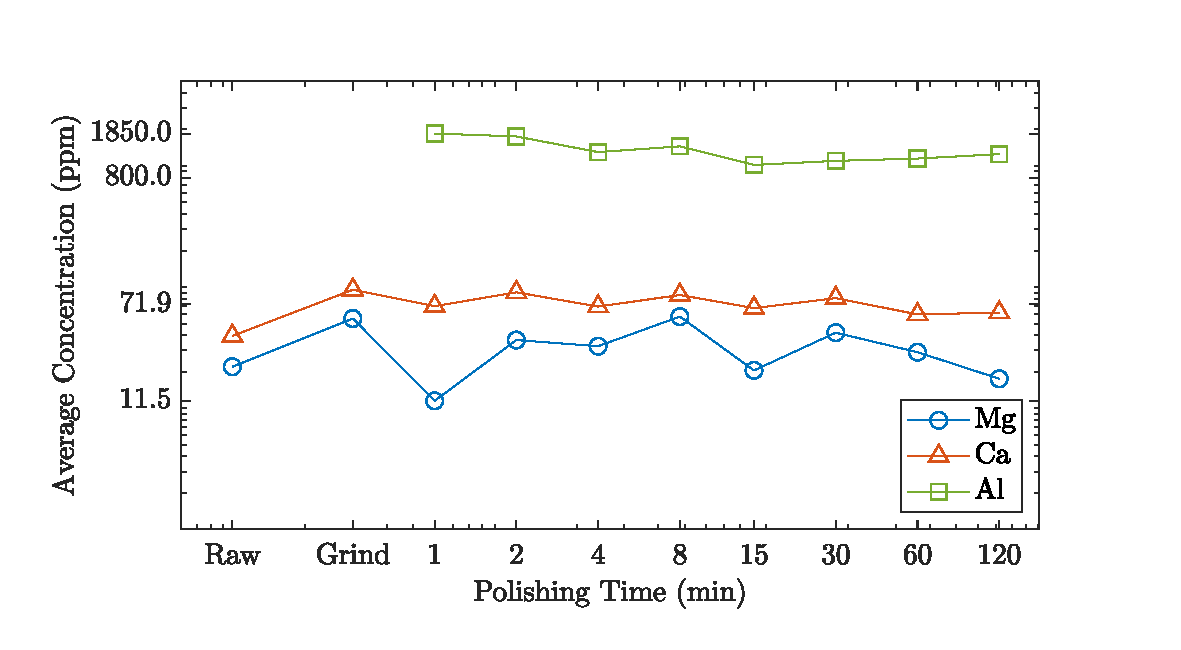
\includegraphics[width = \textwidth]{chapter_5/LIBS/Tap_elem_comparisons/Tap_elements_15_pc.pdf} 
    \vspace*{-30pt}
    \caption{Comparison of the concentration values of the major contaminants as a function of the polishing time, for the glass polished with a 15pc suspension.}
    \label{fig:tap_elem_15pc}
 \end{figure}

 The evolution of the concentrations of the elements is similar to the case presented in the previous section, with only slightly less variation.









 \subsubsection{Polish Concentration: 30pc}
 \label{subsubsec:30pc}
 \vspace*{-25pt}
 \begin{figure}[H]
     \centering
     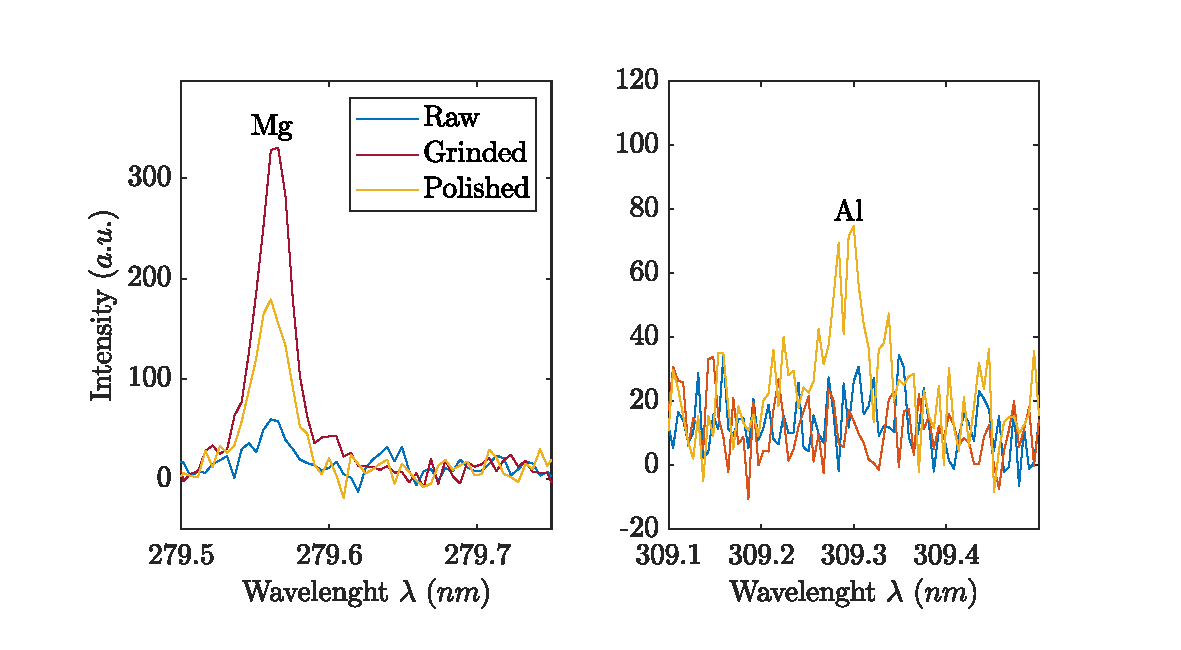
\includegraphics[width = \textwidth]{chapter_5/LIBS/spectra_comparison/tap_30pc_first.pdf} 
     %\caption{Width and depth measurements of LIBS craters performed with a 3D microscope. The peaks are ordered from left to right accordingly to the number of pulses.}
     %\label{fig:3d_microscope_craters}
  \end{figure}
 
 \vspace*{-68pt}
 \begin{figure}[H]
     \centering
     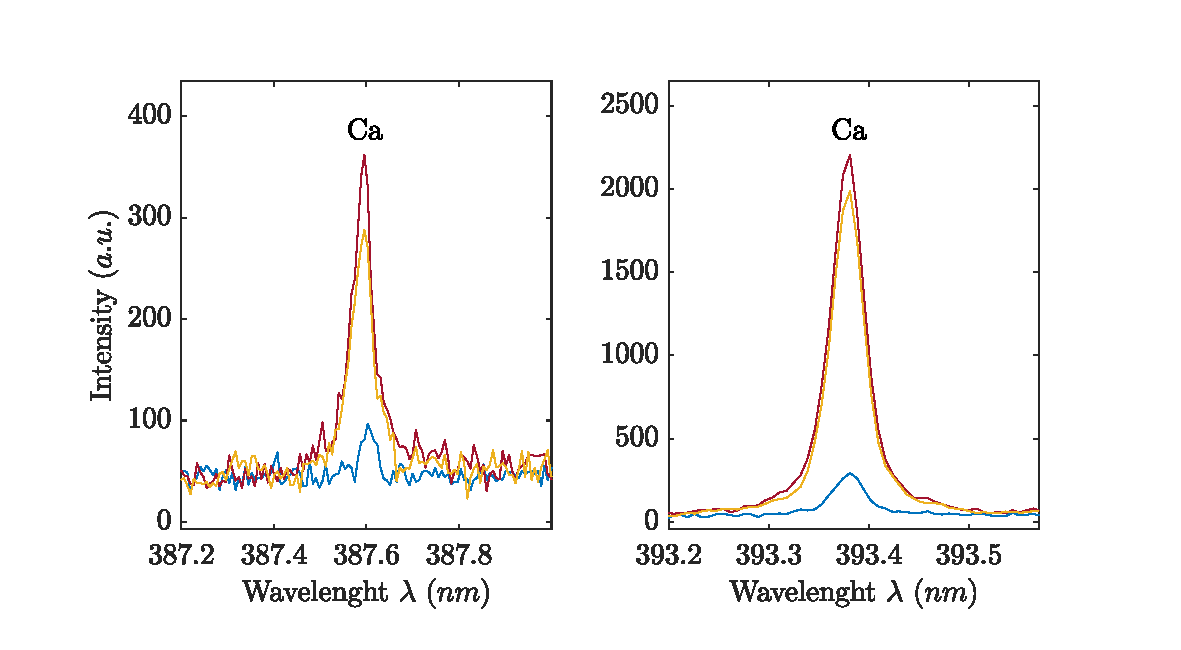
\includegraphics[width = \textwidth]{chapter_5/LIBS/spectra_comparison/tap_30pc_second.pdf} 
     %\caption{Width and depth measurements of LIBS craters performed with a 3D microscope. The peaks are ordered from left to right accordingly to the number of pulses.}
     %\label{fig:3d_microscope_craters}
  \end{figure}
 
 \vspace*{-68pt}
 \begin{figure}[H]
     \centering
     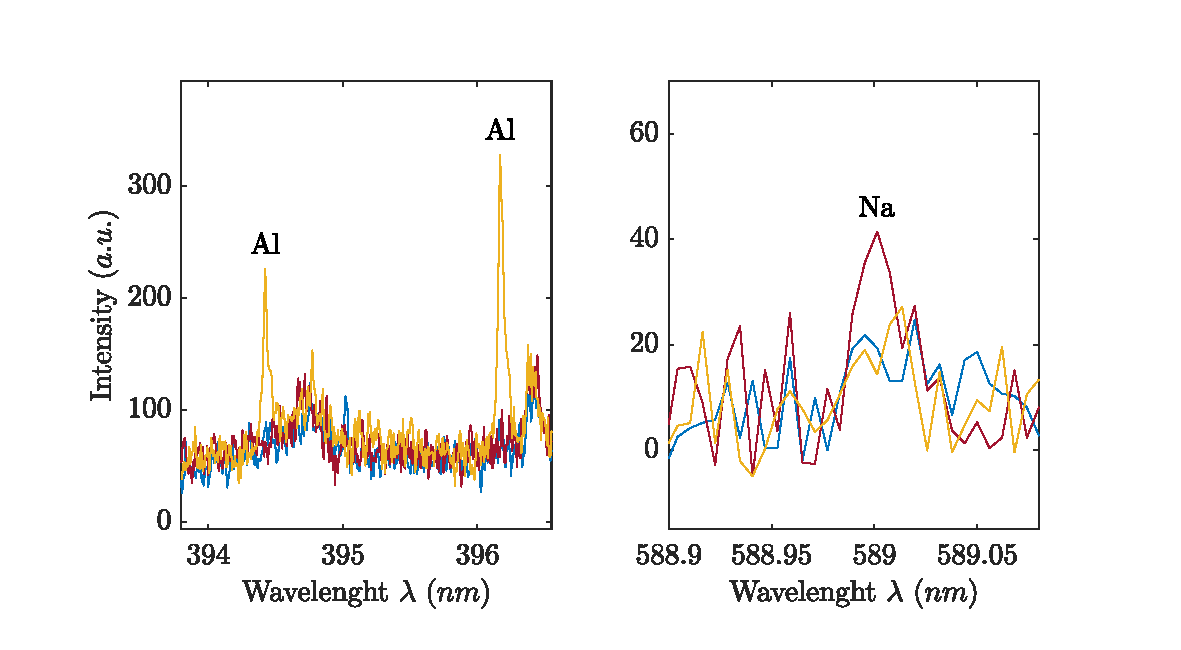
\includegraphics[width = \textwidth]{chapter_5/LIBS/spectra_comparison/tap_30pc_third.pdf} 
     %\caption{Width and depth measurements of LIBS craters performed with a 3D microscope. The peaks are ordered from left to right accordingly to the number of pulses.}
     %\label{fig:3d_microscope_craters}
  \end{figure}
 
From the magnesium and calcium plots, it appears that the concentration of water-related contaminants is much higher in the ground sample. This is confirmed from the Figure~\ref{fig:tap_elem_30pc}, where it is evident that the concentration of those elements is lower at the final stages of polishing.

 \begin{figure}[H]
     \centering
     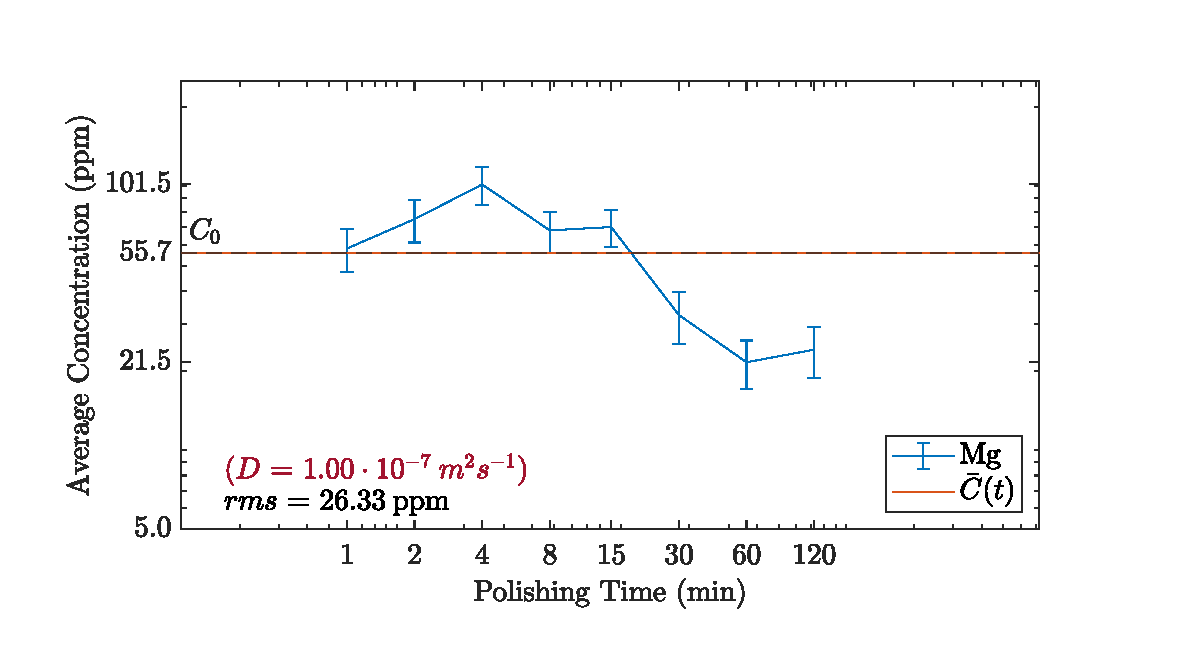
\includegraphics[width = \textwidth]{chapter_5/LIBS/data_fit/fit_tap_30pc_Mg.pdf} 
  \end{figure}
 
  \begin{figure}[H]
     \centering
     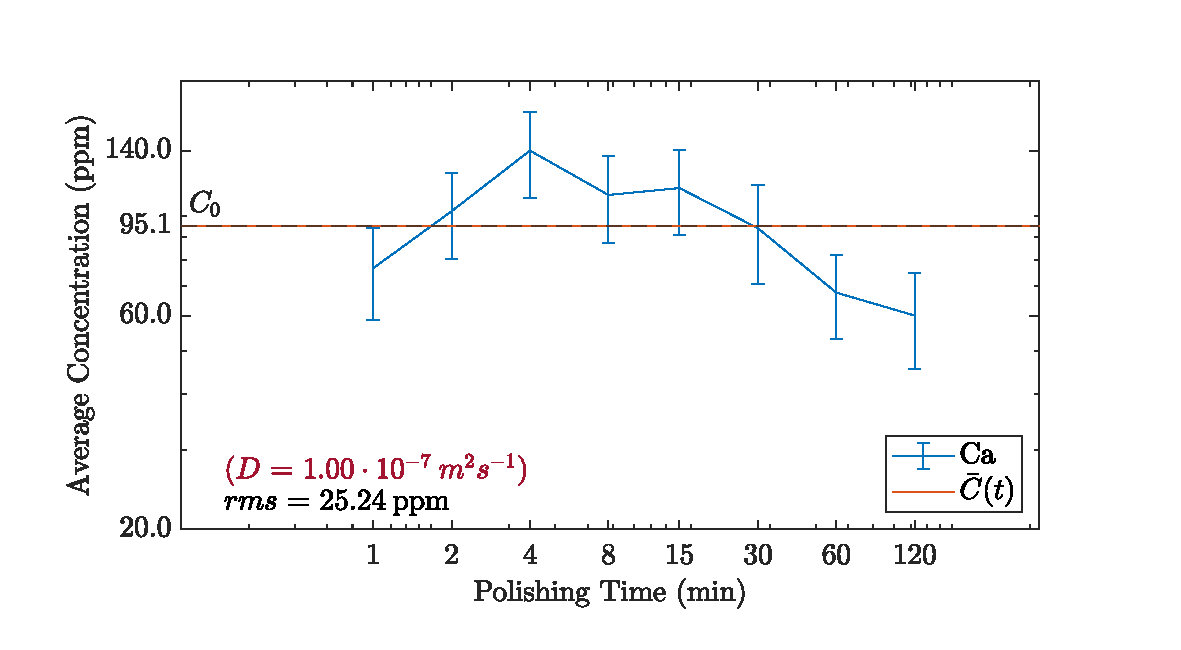
\includegraphics[width = \textwidth]{chapter_5/LIBS/data_fit/fit_tap_30pc_Ca.pdf} 
     %\caption{Width and depth measurements of LIBS craters performed with a 3D microscope. The peaks are ordered from left to right accordingly to the number of pulses.}
     %\label{fig:3d_microscope_craters}
  \end{figure}
     \vspace{-40pt}
  \begin{figure}[H]
     \centering
     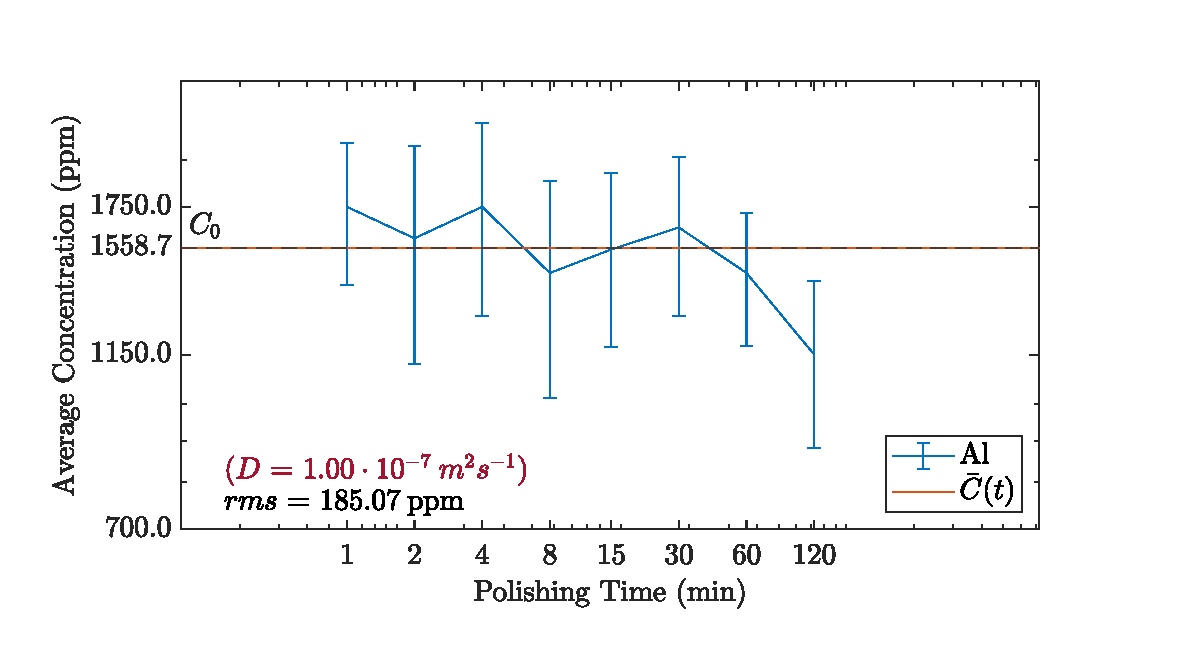
\includegraphics[width = \textwidth]{chapter_5/LIBS/data_fit/fit_tap_30pc_Al.pdf} 
     %\caption{Width and depth measurements of LIBS craters performed with a 3D microscope. The peaks are ordered from left to right accordingly to the number of pulses.}
     %\label{fig:3d_microscope_craters}
  \end{figure}

 
  \begin{figure}[H]
     \centering
     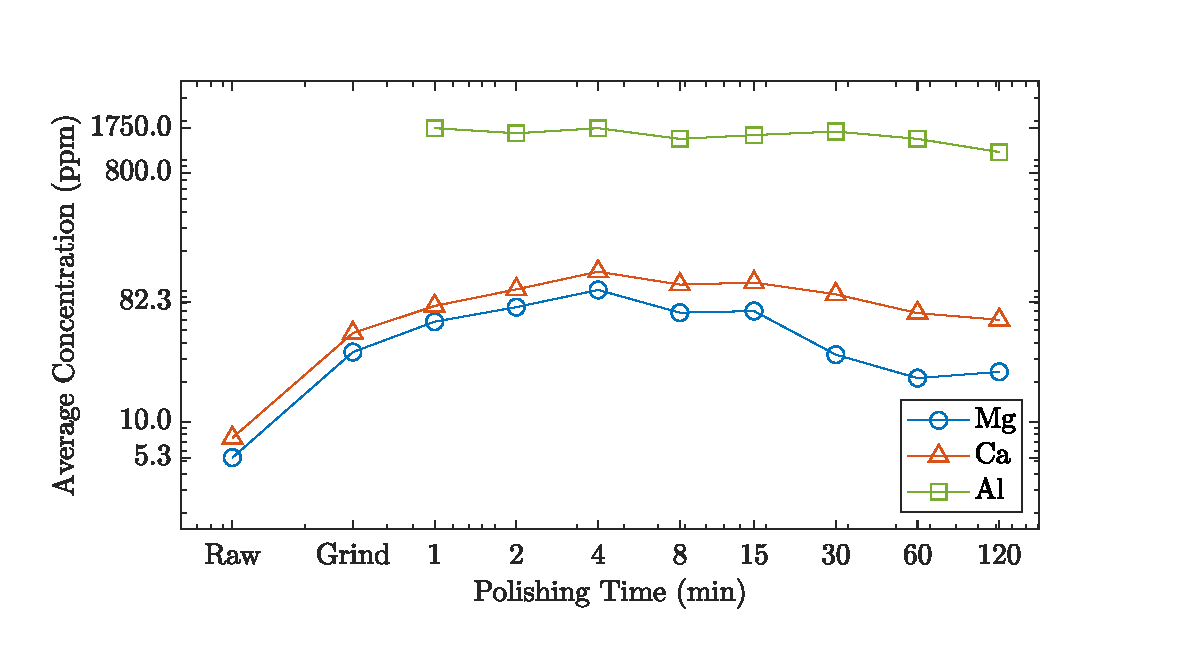
\includegraphics[width = \textwidth]{chapter_5/LIBS/Tap_elem_comparisons/Tap_elements_30_pc.pdf} 
     \vspace*{-30pt}
     \caption{Comparison of the concentration values of the major contaminants as a function of the polishing time, for the glass polished with a 30pc suspension.}
     \label{fig:tap_elem_30pc}
  \end{figure}


\subsubsection{Comparison between Polish Concentrations}
\label{subsubsec:comp_between_pol_conc}


\begin{figure}[H]
   \centering
   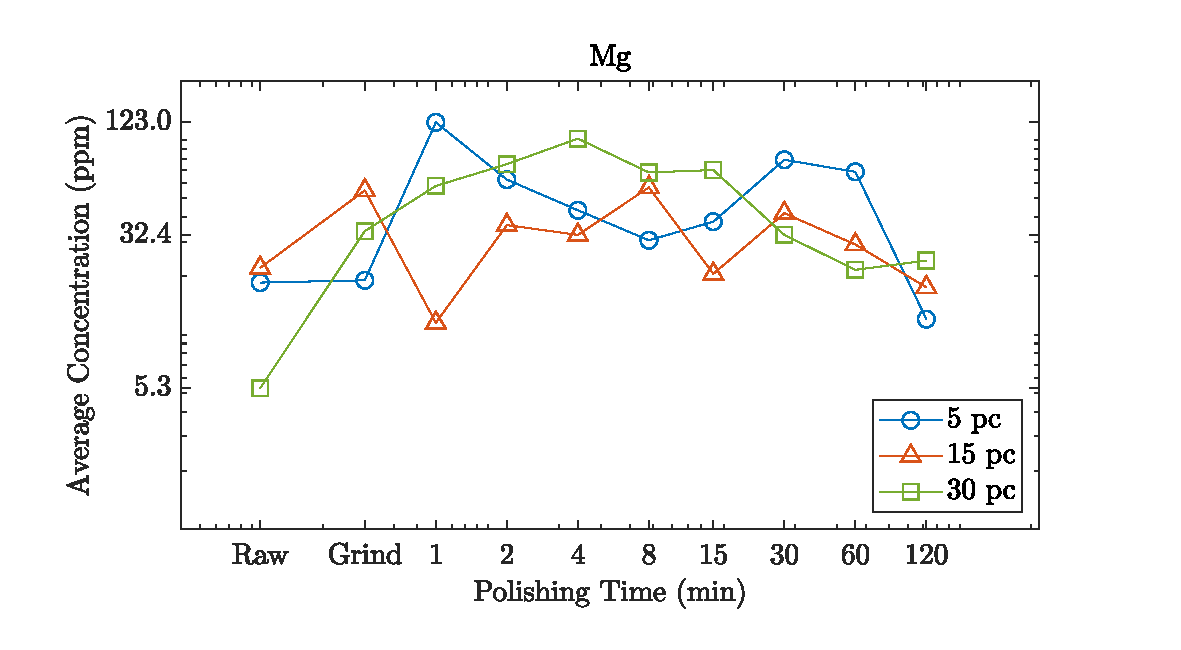
\includegraphics[width = \textwidth]{chapter_5/LIBS/Tap_conc_comparisons/Tap_conc_comp_Mg.pdf} 
   \vspace*{-30pt}
   \caption{Comparison between the magnesium concentrations relative to the different polishing solutions.}
   \label{fig:tap_conc_comp_mg}
\end{figure}

\begin{figure}[H]
   \centering
   \includegraphics[width = \textwidth]{chapter_5/LIBS/Tap_conc_comparisons/Tap_conc_comp_ca.pdf} 
   \vspace*{-30pt}
   \caption{Comparison between the calcium concentrations relative to the different polishing solutions.}
   \label{fig:tap_conc_comp_ca}
\end{figure}

\begin{figure}[H]
   \centering
   \includegraphics[width = \textwidth]{chapter_5/LIBS/Tap_conc_comparisons/Tap_conc_comp_al.pdf} 
   \vspace*{-30pt}
   \caption{Comparison between the aluminum concentrations relative to the different polishing solutions.}
   \label{fig:tap_conc_comp_al}
\end{figure}

The most notable consideration that can be derived from these graphs is that the presence of aluminum on the surface does not seem to have a clear dependence on the concentration of the solution. Moreover, the aluminum appears to have a more evident decreasing behavior respect to the other contaminants. This could be partially related to the fact that alumina is not soluble, unlike, for example, calcium carbonate which should be the main cause of the presence of calcium.
\\
More details on this hypothesis will be presented in the conclusions.

\subsection{Different Types of Water}
\label{subsec:different_type_of_water}

With a similar structure to the previous section, here will be presented the results of the measurements carried out with distilled water. The concentration of the polishing suspension is 15pc.

\begin{figure}[H]
    \centering
    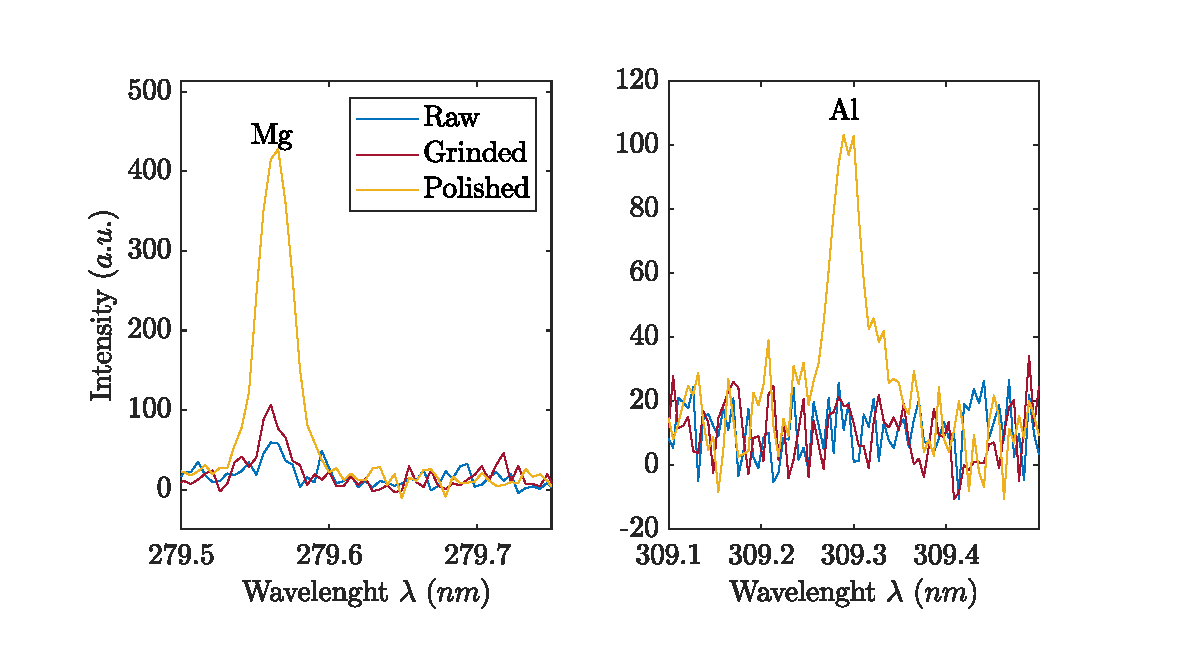
\includegraphics[width = \textwidth]{chapter_5/LIBS/spectra_comparison/dist_15pc_first.pdf} 
    %\caption{Width and depth measurements of LIBS craters performed with a 3D microscope. The peaks are ordered from left to right accordingly to the number of pulses.}
    %\label{fig:3d_microscope_craters}
 \end{figure}

\vspace*{-68pt}
\begin{figure}[H]
    \centering
    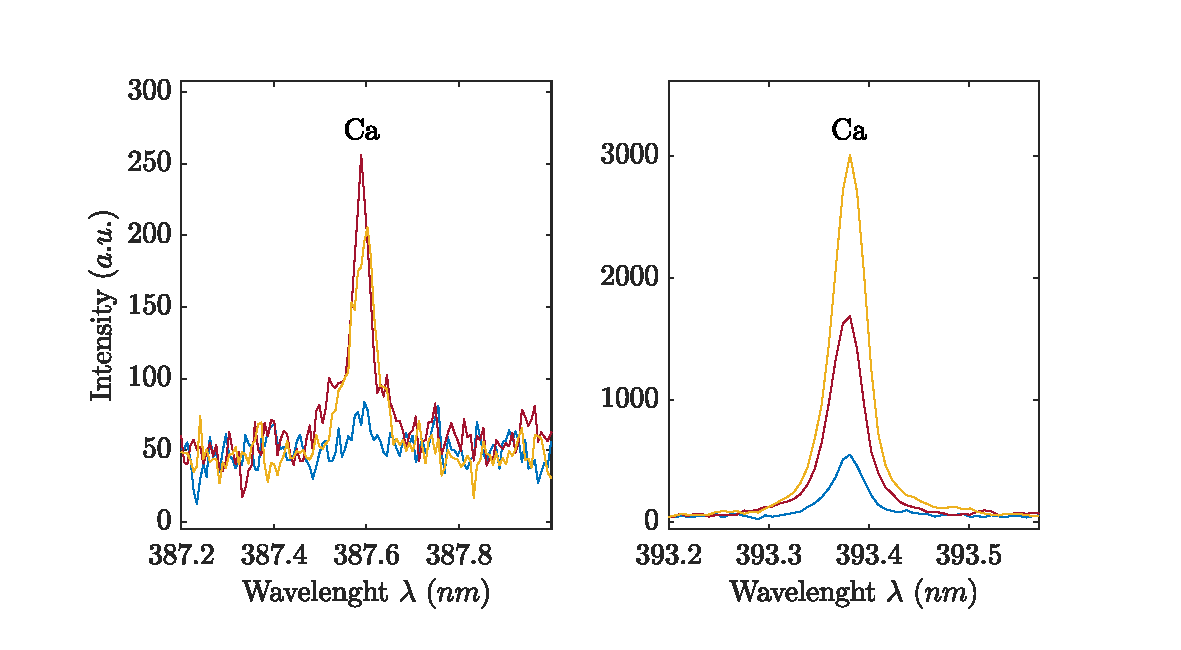
\includegraphics[width = \textwidth]{chapter_5/LIBS/spectra_comparison/dist_15pc_second.pdf} 
    %\caption{Width and depth measurements of LIBS craters performed with a 3D microscope. The peaks are ordered from left to right accordingly to the number of pulses.}
    %\label{fig:3d_microscope_craters}
 \end{figure}

\vspace*{-68pt}
\begin{figure}[H]
    \centering
    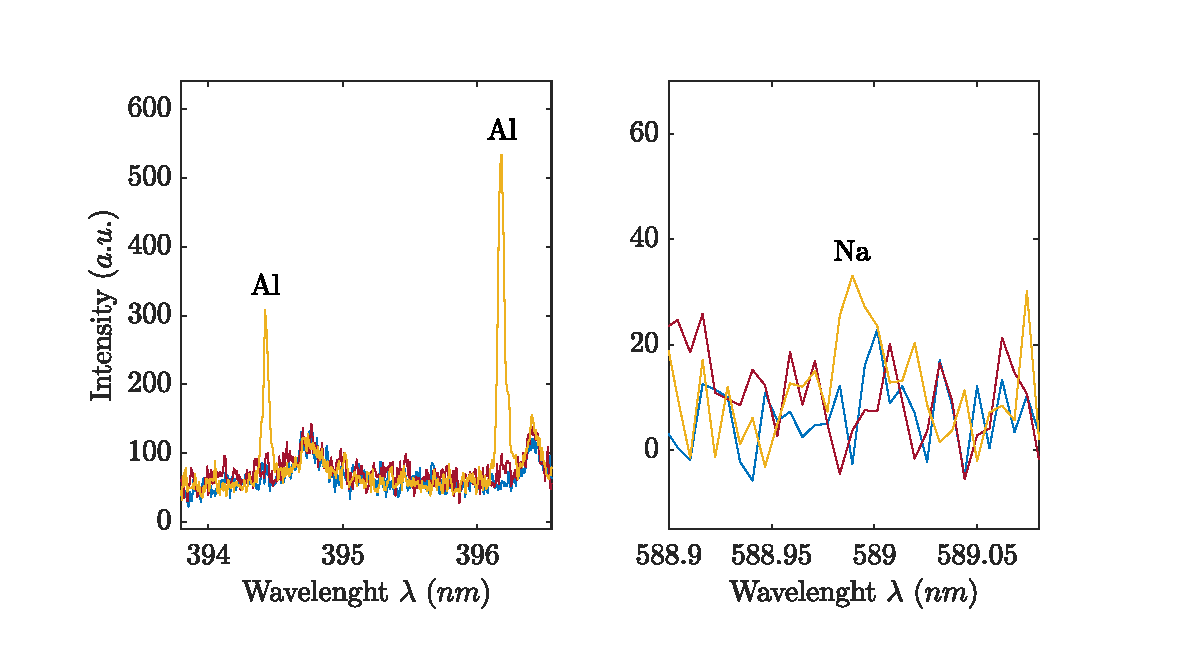
\includegraphics[width = \textwidth]{chapter_5/LIBS/spectra_comparison/dist_15pc_third.pdf} 
    %\caption{Width and depth measurements of LIBS craters performed with a 3D microscope. The peaks are ordered from left to right accordingly to the number of pulses.}
    %\label{fig:3d_microscope_craters}
 \end{figure}


 \begin{figure}[H]
    \centering
    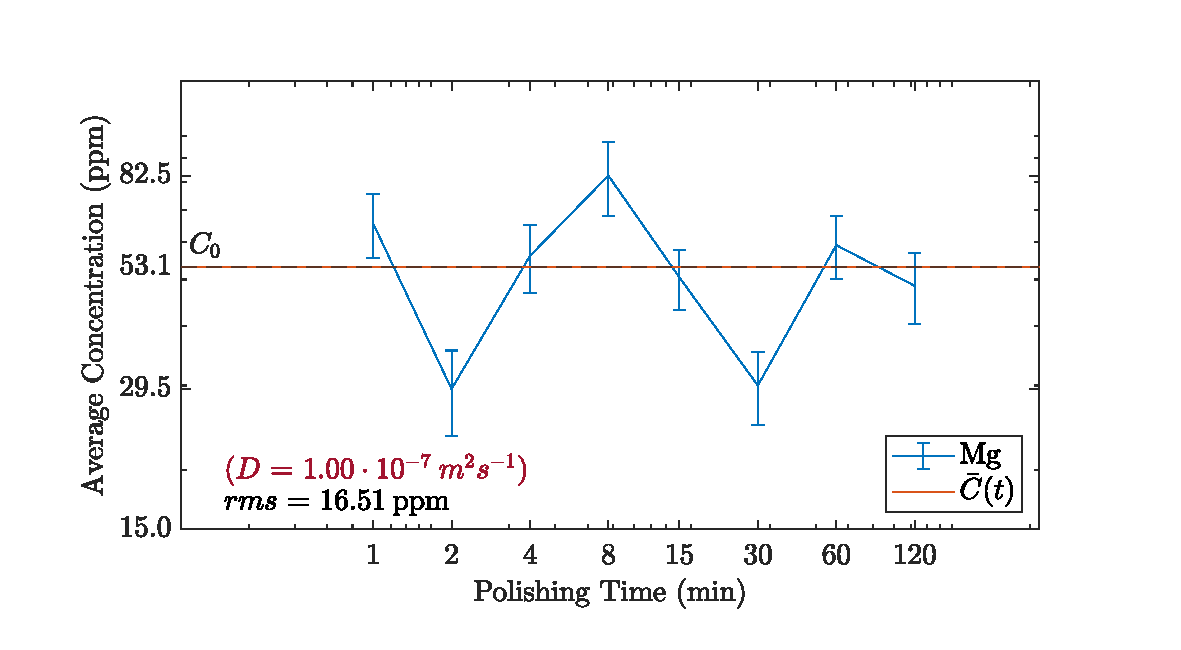
\includegraphics[width = \textwidth]{chapter_5/LIBS/data_fit/fit_dist_15pc_Mg.pdf} 
 \end{figure}

 \begin{figure}[H]
    \centering
    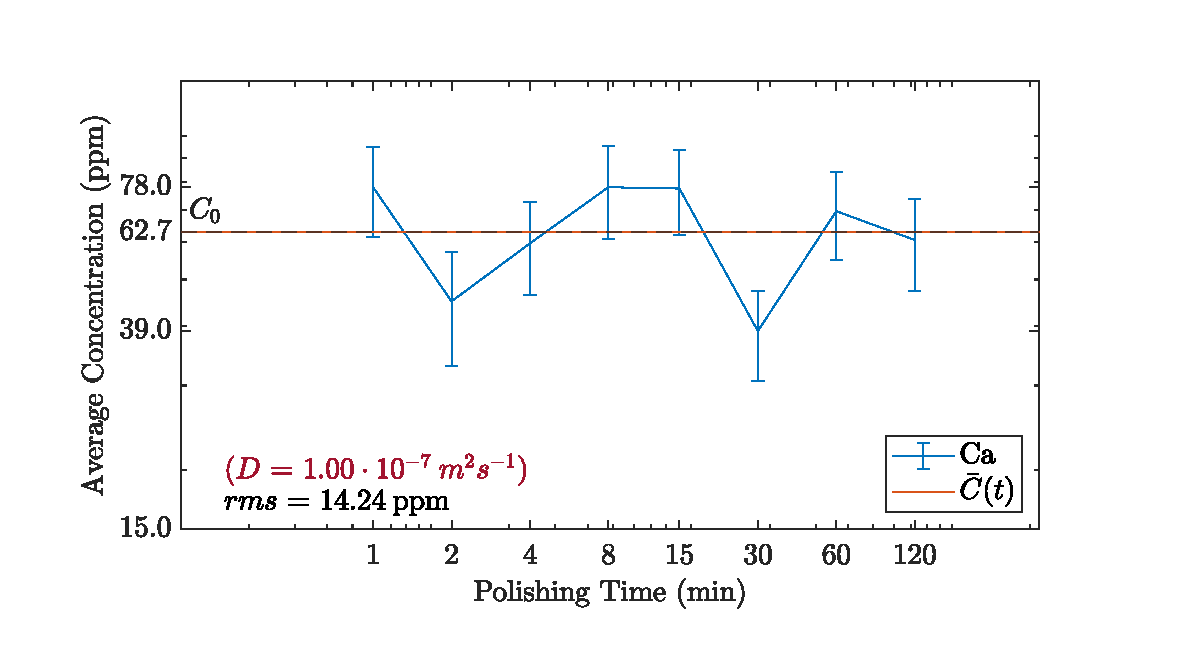
\includegraphics[width = \textwidth]{chapter_5/LIBS/data_fit/fit_dist_15pc_Ca.pdf} 
    %\caption{Width and depth measurements of LIBS craters performed with a 3D microscope. The peaks are ordered from left to right accordingly to the number of pulses.}
    %\label{fig:3d_microscope_craters}
 \end{figure}
    \vspace{-40pt}
 \begin{figure}[H]
    \centering
    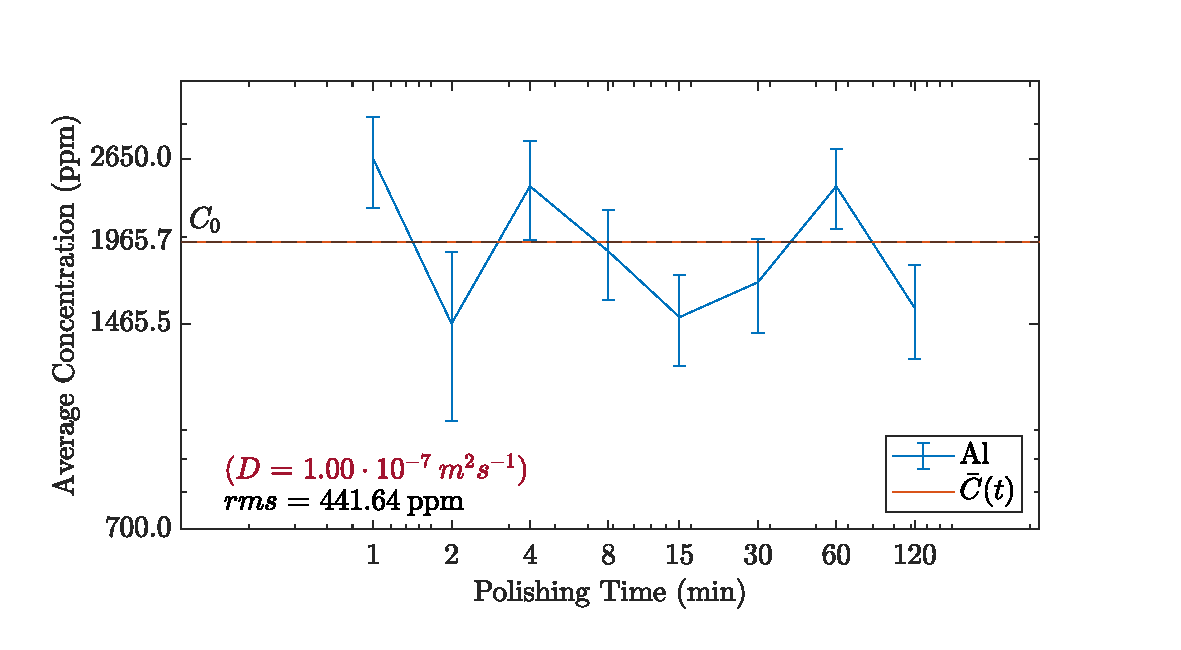
\includegraphics[width = \textwidth]{chapter_5/LIBS/data_fit/fit_dist_15pc_Al.pdf} 
    %\caption{Width and depth measurements of LIBS craters performed with a 3D microscope. The peaks are ordered from left to right accordingly to the number of pulses.}
    %\label{fig:3d_microscope_craters}
 \end{figure}

CALCIUM 30PC DA RIFARE